\documentclass[11pt,a4paper]{report}

%------------ package pour langue fr ------
\usepackage[utf8]{inputenc}
\usepackage[french]{babel}
\usepackage[T1]{fontenc}
\usepackage{multicol}
\usepackage{enumitem}
%------------- for embedding images----------
\usepackage{graphicx} 
\usepackage{float}
\usepackage[export]{adjustbox}
\usepackage{amsfonts,epsfig,epstopdf,titling,url,array}

\usepackage{amsmath}
\usepackage{amssymb}
\usepackage{amsthm}
%%algorithme
\usepackage{algorithm}
\usepackage[noend]{algpseudocode}
%--------- pour le style de la page ----------
%\usepackage[top=2cm, bottom=2cm, right=2cm, left=2cm]{geometry}
\usepackage[]{geometry}
\usepackage{setspace}
\setstretch{1,5}
%\usepackage{txfonts} //pour utiliser times new roman dans le document
\usepackage{fancyhdr}
\pagestyle{fancy}
\renewcommand\headrulewidth{1pt}
\fancyhead[L]{Bousbiat Hafsa - Ihadadene Sana}
\fancyhead[R]{Rapport Master}
%--------------------------- Sommaire ----------------------------%
\usepackage{hyperref}
\usepackage{amssymb}
\usepackage{natbib}
\theoremstyle{definition}
		\newtheorem{defn}{Definition}[section]
		\newtheorem{conj}{Conjecture}[section]
		\newtheorem{exmp}{Example}[section]
\begin{document}

%Page de garde (page de titre)							Obligatoire

\begin{titlepage}

\newgeometry{top=0mm,right=20mm,left=20mm,bottom=0mm}



	%--------------------  Entete de l'Ecole ----------------------%

	\begin{figure}[t]
		
\includegraphics[scale=0.75]{./ressources/image/ESI.png}\\[0.6in]
	\end{figure}
	
	
	
	%--------------------------------------------------------------%
	\begin{center}
	
	%------------------------  Le sujet ---------------------------%
		\LARGE \textbf{ Mémoire}\\
		\Large{
			Pour Obtention du diplôme de Master En Informatique\\
			\textbf{Option : Système Informatique (SIQ)}
			%\textsc thèse D'Ingéniorat En Informatique sous le thème :
		}\\[0.2in]
		\huge {
		\rule{\linewidth}{.5pt}
			\textbf{
				Étude et classification des méthodes de compression de graphe par extraction de motifs et k2-trees
			} 
			\rule{\linewidth}{.5pt}
		}\\[0.5in]
		\Large
	%--------------------------------------------------------------%	
	
	%-------------------------  Mon nom ---------------------------%
	\textbf{Réaliser par:}\\
	\begin{multicols}{2}
			\Large 	Mlle. Hafsa Bousbiat\\
			\large eh\_bousbiat@esi.dz\\
			ESI\\
		\columnbreak
 			\Large Mlle. Sana Ihadadene\\
			\large es\_ihadadene@esi.dz\\
			ESI \\
		
	\end{multicols} 
	
	\vskip 0.1in
	%--------------------------------------------------------------%	

	%-----------------------  Encadreures -------------------------%
	 \textbf{Encadrer par:}\\
	 
	 \begin{multicols}{2}
			\Large 	Dr. Karima Amrouche\\
			\large k\_amrouche@esi.dz\\
			ESI\\
		\columnbreak
 			\Large Dr. Hamida Seba\\
			\large hamida.seba@univ-lyon1.fr\\
			Université de Lyon \\
	\end{multicols}
	
	%--------------------------------------------------------------%	
	
	\small
	\vskip 0.3in
	Octobre 2018 \\
	Année Universitaire: 2018-2019\\
	
	\end{center}		
\restoregeometry
\end{titlepage}

%Remerciements											Obligatoire
\begin{center}
	\par
	\textit{
		\vskip 1in
		\Huge 
			Remerciement \\[0.5in]
			\addcontentsline{toc}{chapter}{\numberline{}Remerciement}
	}
\end{center}
	\par
  Nous tenons d'abord à exprimer notre gratitude à l'égard de nos encadrants, Madame Seba
Hamida, Madame Amrouche Karima et Monsieur Mohammed pour leur précieuse	aide, leur judicieux conseils  et pour le temps qu'ils nous ont consacré tout au long de ce PFE.\\


Nous remercions également toute l'équipe pédagogique de l'École Nationale
Supérieure d'Informatique, et à leur tète les enseignants pour la richesse et la qualité de la formation qu'ils nous ont offert tout au long de notre cursus.\\


Nous tenons à remercier les membres du jury qui nous ont fait l’honneur d’accepter de juger
cet humble travail.\\


Enfin, nous adressons nos plus sincères remerciements à tous nos proches et amis, qui nous ont toujours encouragée au cours de la réalisation de ce mémoire.
Merci à tous et à toutes.

\newpage
 


%Résumé												Obligatoire
\begin{center}
	\par
	\textbf{
		\vskip 0.5in
		\LARGE 
			Résumé \\[0.15in]
			\addcontentsline{toc}{chapter}{\numberline{}Résumé}
	}
\end{center}
	\par
    Lorem ipsum dolor sit, amet consectetur adipisicing elit. Nostrum tempore ea fugiat numquam autem saepe quas porro vitae? Fugit commodi tempore voluptate sint fugiat, possimus optio ad! Pariatur, obcaecati quidem.
Lorem ipsum dolor, sit amet consectetur adipisicing elit. Neque excepturi ducimus accusantium eius voluptatibus, quod velit, explicabo tenetur aliquid ipsam sapiente. Quibusdam quis ullam, saepe numquam molestias nobis recusandae labore?    Lorem ipsum dolor sit, amet consectetur adipisicing elit. Nostrum tempore ea fugiat numquam autem saepe quas porro vitae? Fugit commodi tempore voluptate sint fugiat, possimus optio ad! Pariatur, obcaecati quidem.
Lorem ipsum dolor, sit amet consectetur adipisicing elit. Neque exceptu 

\begin{center}
	\par
	\textbf{
		\vskip 0.5in
		\LARGE 
			Abstract \\[0.15in]
	}
\end{center}
	\par
    Lorem ipsum dolor sit, amet consectetur adipisicing elit. Nostrum tempore ea fugiat numquam autem saepe quas porro vitae? Fugit commodi tempore voluptate sint fugiat, possimus optio ad! Pariatur, obcaecati quidem.
Lorem ipsum dolor, sit amet consectetur adipisicing elit. Neque excepturi ducimus accusantium eius voluptatibus, quod velit, explicabo tenetur aliquid ipsam sapiente. Quibusdam quis ullam, saepe numquam molestias nobis recusandae labore?    Lorem ipsum dolor sit, amet consectetur adipisicing elit. Nostrum tempore ea fugiat numquam autem saepe quas porro vitae? Fugit commodi tempore voluptate sint fugiat, possimus optio ad! Pariatur, obcaecati quidem.
Lorem ipsum dolor, sit amet consectetur adipisicing elit. Neque exceptu

\newpage

%Sommaire (Table des matières)							Obligatoire
\tableofcontents
\newpage

%Liste des figures										Selon besoin
\listoffigures
\addcontentsline{toc}{chapter}{\numberline{}Liste des figures}
\cleardoublepage

%Liste des tableaux										Selon besoin

\listoftables
\addcontentsline{toc}{chapter}{\numberline{}Liste des tableaux}
\cleardoublepage

%Introduction (début de la pagination)					bligatoire


\part{Introduction} 


%---->chapitre 01 :« cadrage du projet »
	\chapter{ Théorie des graphes}
	  Pour faciliter la compréhension d'un problème, nous avons tendance à  le dessiner ce qui nous amène parfois même à le résoudre. La théorie des graphes est fondée à l'origine sur ce principe. De nombreuses propriétés et méthodes ont été pensées ou trouvées à partir d'une représentation schématique pour être ensuite formalisées et prouvées.


La théorie des graphes est historiquement un domaine mathématique qui s'est développé  au sein des autres disciplines comme la chimie, la biologie, la sociologie et l'industrie. Elle constitue aujourd'hui un corpus de connaissance très important et un instrument efficace pour résoudre une multitude de problèmes.


De manière générale, le graphe sert à représenter les structures, les connexions entre différents composants, les acheminements possibles pour un ensemble complexe composé d'un grand nombre de situations en exprimant les dépendances et les relations entre ses éléments,(e.g. réseau routier ou ferroviaire, réseau de communication, diagramme d'ordonnancement, ..). 


Dans ce chapitre, nous présenterons les notions et les concepts clés relatives aux graphes qui serviront de base pour la suite de notre travaille, à savoir : la définition d'un graphe, ses types et sa représentation structurelle. Nous clôturons le chapitres avec quelques domaines d'application des graphes.

	
	\section{Graphe non orienté}
			\subsection{Définitions et généralités}
		
Un graphe non orienté G est la donnée d’un couple (V , E) où V = \{$ \textit{v}_{1} , \textit{v}_{2} ,..., \textit{v}_{n} $\} est un ensemble fini dont les éléments sont appelés sommets ou nœuds ( Vertices en anglais ) et  E=\{$\textit{e}_{1} ,  \textit{e}_{2} ,…, \textit{e}_{m} $\} est un ensemble fini d'arêtes ( Edges en anglais ). Toute arête \textit{e} de E correspond à un couple non ordonné de sommets ( $\textit{v}_{i} , \textit{v}_{j}$ ) $\in$ E $\subset$  $V \times V$ représentant ses extrémités \citep{muller} \citep{fages2014exploitation}.
\\Soient \textit{e} = ($\textit{v}_{i} , \textit{v}_{j}$) et \textit{e'}=($\textit{v}_{k} , \textit{v}_{l}$) deux arêtes de E, On dit que :
\begin{itemize}
\item $\textit{v}_{i}$ et $\textit{v}_{j}$ sont les extrémités de \textit{e} et \textit{e} est incidente à $\textit{v}_{i}$ et $\textit{v}_{j}$ \citep{hennecart2012elements}.
\item $\textit{v}_{i}$ et $\textit{v}_{j}$ sont voisins ou adjacents, s'il y a au moins une arête entre eux dans E \citep{IUTLyonInformatique}.
\item L'ensemble des sommets adjacents aux deux extrémités de \textit{e} est appelé le voisinage de \textit{e} \citep{muller}. 
\item \textit{e} et \textit{e'} sont voisins s'ils ont une extrémité commune  \citep{lopez2003cours}.
\item L'arête \textit{e} est une boucle si ses extrémités coïncident, i.e, $\textit{v}_{i}$ = $\textit{v}_{j}$ \citep{IUTLyonInformatique}. 
\item L'arête \textit{e} est multiple si elle a plus d'une seule occurrence dans l'ensemble E.
\end{itemize}	
		 
\subsection{Représentation graphique}
Un graphe non orienté G peut être représenté par un dessin sur un plan comme suit \citep{muller}:

\begin{itemize}
\item Les nœuds $\textit{v}_{i}$ $\in$ V de G sont représentés par des points distincts.
\item 	Les arêtes \textit{e} = ($\textit{v}_{i}$,$\textit{v}_{j}$) $\in$ E de G sont représentés par des lignes, pas forcement rectilignes, qui relient les extrémités de chaque arête \textit{e}.
\end{itemize}

%% L'exemple de la représentation graphique 
\textbf{Exemple :}
 Soit g=(V1 , E1) un graphe non orienté tel que : V1=\{ 1,2,3,4,5 \} et E1=\{(1,2), (1,4), (2,2), (2,3), (2,5), (3,4)\}.
La représentation graphique de g est alors donnée par le schéma de la figure \ref{graphNonOriente}.
\\
\begin{figure}[H]
\begin{center}
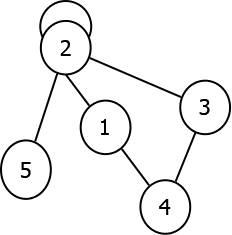
\includegraphics[height=120 pt, width=130 pt]{./ressources/image/graphNonOriente.png} 
\end{center}
\caption{Exemple de représentation graphique d'un graphe non orienté}
\label{graphNonOriente}
\end{figure}

		\subsection{Propriétés d'un graphe}
		
		\begin{itemize}[label=$\circ$]
			
			\item \textbf{Ordre d'un graphe:} On appelle ordre d’un 					graphe le nombre de ses sommets, i.e, Card(V) \citep{DUT}.
			
			\item  \textbf{Taille d'un graphe:} On appelle taille d’un 				graphe le nombre de ses arêtes, i.e, Card(E) \citep{DUT}.
			
			\item  \textbf{Degré dans un graphe:}
			
			
			\begin{itemize}[label=$\bullet$]
				\item \textbf{Degré d'un sommet : } Le degré d’un sommet noté \textit{d}($\textit{v}_{i}$) est le nombre d'arêtes incidentes à ce sommet, sachant qu’une boucle compte pour deux \citep{muller}. Dans l'exemple de la figure \ref{graphNonOriente}, le degré du sommet (1) est : \textit{d}(1)=2.
				
				\item \textbf{Degré d'un graphe : }Le degré d’un graphe est le degré maximum de ses sommets, i.e, max(\textit{d}($\textit{v}_{i}$)) \citep{muller}. Dans l’exemple de 				la figure \ref{graphNonOriente}, le degré du graphe g est \textit{d}(2)=5.
			\end{itemize}
			
			\item \textbf{Rayon et diamètre dans un graphe:}
			\begin{itemize}[label=$\bullet$]
				\item \textbf{Distance : }La distance entre deux sommets 	\textit{v} et \textit{u} est le plus petit nombre d’arêtes qu’on doit parcourir pour aller de \textit{v} à \textit{u} ou de \textit{u} à \textit{v} \citep{muller}. 
				
				\item 	\textbf{Diamètre d’un graphe :} C’est la plus grande 	distance entre deux sommets de ce graphe \citep{muller}. 
				
				\item 	\textbf{Rayon d’un graphe : }C’est la plus petite distance entre deux sommets de ce graphe \citep{parlebas1972centralite}. 
			\end{itemize}
		\end{itemize}
		
	
			
	
			
	\section{Graphe orienté}	
		
		\subsection{Définitions et généralités}
		Un graphe orienté G est la donnée d'un couple (V , E) où
		V est un ensemble fini dont les éléments sont appelés les sommets de G et 
		E  $\subset$ V x V est un ensemble de couples ordonnés de sommets dits arcs ou arêtes \citep{muller}. G est appelé dans ce cas digraphe (directed graph).\\
		 Pour tout arc e = ( $v_{i}$ , $v_{j}$) $\in$ E :
		 \begin{itemize}  
			\item $v_{i}$ est dit extrémité initiale ou origine de e et $v_{j}$ est l'extrémité finale de e \citep{muller}.
			
			\item $v_{i}$ est le prédécesseur de $v_{j}$ et $v_{j}$ est le successeur de $v_{i}$ \citep{IUTLyonInformatique}.
			
			\item les sommets $v_{i}$ , $v_{j}$ sont des sommets adjacents \citep{Pres}.
			
			\item e est dit sortant en $v_{i}$ et incident en $v_{j}$ \citep{Pres}.
			
			\item e est appelé boucle si $v_{i}$ = $v_{j}$, i.e l'extrémité initiale et finale représente le même sommet \citep{IUTLyonInformatique}.
			
		\end{itemize}
		 
		
		\subsection{Représentation graphique}
		
		
		Un graphe G = (V , E) peut être projeter sur le plan en représentant:
		\begin{itemize} 
		\item Dans un premier temps les nœuds $v_{i}$ $\in$ V par des points disjoints du plan.
		\item Et dans un second temps les arêtes e = ( $v_{i}$ , $v_{j}$) $\in$ E par des lignes orientées reliant par des flèches les deux extrémités de e. 
		\end{itemize}
		
		\textbf{Exemple:}
		
		Soit g = ($V_{1}$ , $E_{1}$) un digraphe tel que : $V_{1}$ = \{ 1,2,3,4 \} et  $E_{1}$ = \{(1,2),(1,3),(3,2),(3,4),(4,3)\}.
		
		Le représentation graphique de g est alors donné par le schéma de la figure \ref{grapheOr}.
	
		
			\begin{figure}[h]
			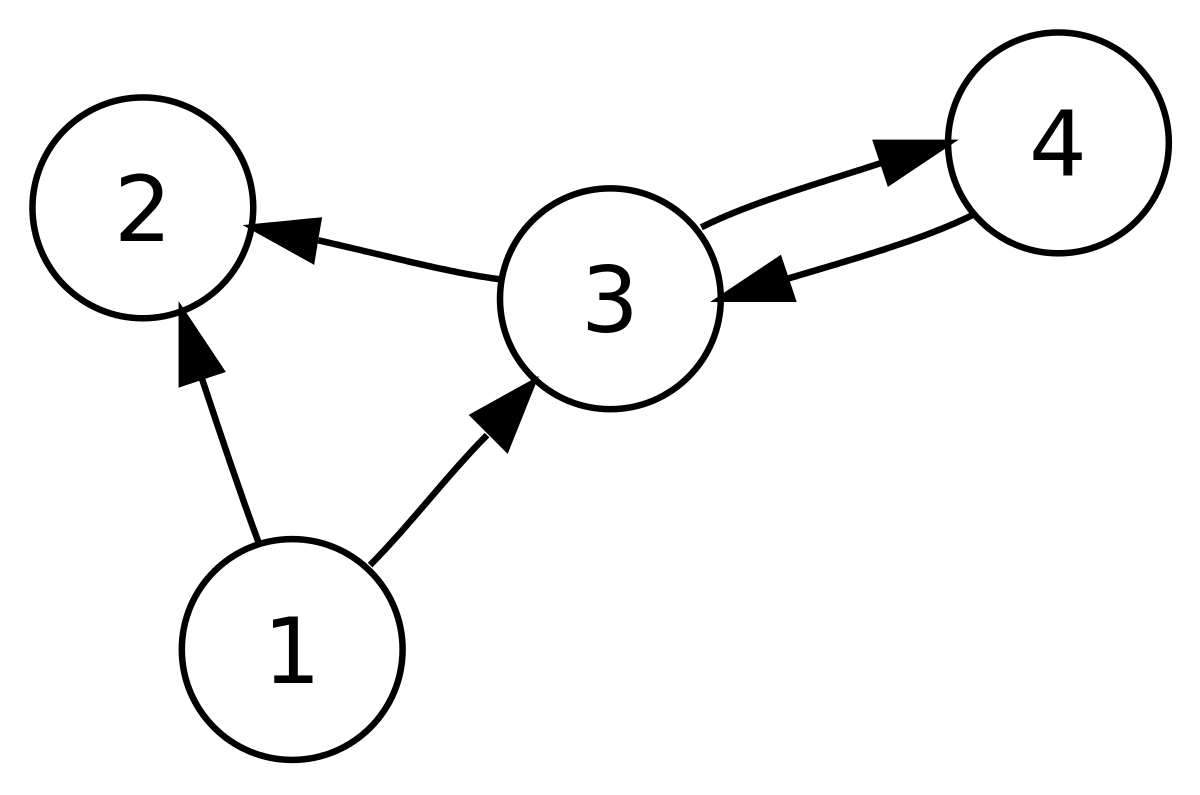
\includegraphics[scale=0.15,center]{./ressources/image/RepDiGraphe.png}
			\caption[Exemple de représentation graphique d'un digraphe.]{Exemple de représentation graphique d'un digraphe.}
			\label{grapheOr}
			\end{figure}
			
		
		\subsection{Quelques Propriétés:} %%% Arevoire 
			\begin{itemize}[label=$\circ$]
			\item\textbf{Ordre d'un digraphe:}
			est le nombre de sommets n = Card(V) \citep{DUT}.
			
			\item\textbf{taille d'un digraphe:} est le nombre d’arcs m = Card(A) \citep{DUT}.
			
			\item\textbf{Degré dans un digraphe:}
			Le degré d'un sommet $v_{i}$ $\in$ V dans un digraphe G=(V , E) est donnée par la formule :
			\begin{center}
				d($v_{i}$) = $d^+(v_{i}$) + $d^-(v_{i}$\\
			\end{center}			 
			 où $d^+(v_{i}$) est le nombre d'arcs sortants au sommet $v_{i}$ et est appelé degré extérieure et $d^-(v_{i}$) représente le nombre d'arcs incidents et est appelé degré intérieur \citep{muller}.
			 
			 \item\textbf{Voisinage dans un digraphe:}
			 Le voisinage d'un sommet $v_{i}$ $\in$ V, noté V($v_{i}$), dans un digraphe G = (V , E) est:
			 	\begin{center}
				V($v_{i}$) = succ($v_{i}$) $\bigcup$ pred($v_{i}$),
				\end{center}
				
				où succ($v_{i}$) est l'ensemble des successeurs de $v_{i}$ et pred($v_{i}$) est l'ensemble de ses prédécesseurs \citep{bac}, i.e le voisinage de $v_{i}$ est l'ensemble des sommets qui lui sont adjacents.
			
			\end{itemize}
			
		
	\section{Notion de Connexité}
	
	Les structures de graphes sont généralement exploitables à travers leurs interrogation qui permet de fournir des réponses aux problèmes modélisés. L'un des informations les plus importantes dans un graphe est la notion des relations (indirectes ou indirecte) entre deux nœuds ou plus formellement la connexité dans un graphe. Dans cette partie nous allons définir les concepts relatives à cette notion.
	
	\begin{itemize} [label = $\bullet$]
		
			 
			 \item \textbf{Chemin (resp. Chaine):}
			est une liste de sommets S= $(v_{0},v_{1},v_{2},...,v_{k})$ telle qu’il existe un arc (resp. une arête) entre chaque couple de sommets successifs.
			 
			 
			  \item \textbf{Cycle (resp. Circuit):} 
			 est un chemin (resp. chaine) dont le premier et le dernier sommet sont identiques \citep{DUT}.
			 
			 		\item \textbf{Graphe connexe:}
			Un graphe non orienté (resp. orienté) est dit connexe (resp. fortement connexe) si pour tout pair de sommets ($v_{i}$, $v_{j}$) il existe un chemin S les reliant \citep{muller}.
			 
		\end{itemize}
	
	
	
	\section{Graphe partiel et sous graphe:}
    		
	La quantité de données disponible aujourd'hui et sa croissance de manière exponentielle ont favorisé la décomposition des graphes en des entités plus petites afin de garantir une facilité de compréhension et d'analyse dans le but d'extraire l'information la plus pertinente. Dans cette partie, nous allons définir de manière plus formelle ce que ces entités sont, ainsi que leurs types.
	
		
		
		
		\subsection{Définitions:}
		Soient G = (V , E), $G' = (V' , E')$ et $G'' = (V'' , E'')$ trois graphes.
		\begin{itemize}[label=$\circ$]
		
			\item Le graphe $G'$ est appelé \textbf{graphe partiel} de G si : $V' = V\ et\ E' \subset$ E \citep{DUT}. En d'autres termes, un graphe partiel est obtenu en supprimant une ou plusieurs arêtes de G.
				

			\item Le graphe $G''$ est dit \textbf{sous-graphe} de G si: $V''\subset V$ et 
			 $E''\subset E \cap (V'' x V'')$ \citep{bac}, i.e, un sous-graphe est obtenu en enlevant un ou plusieurs nœuds du graphe initial ainsi que les arêtes dont ils représentent l'une des deux extrémités.
			 
		\end{itemize}
		
		\subsection{Quelques Types de sous graphes:}
		
		\begin{itemize} [label = $\bullet$]
		
		
			\item \textbf{Une Clique :} est un sous-graphe complet de G \citep{bac}.
			
			\item \textbf{Biparti :} G' est un sous-graphe biparti si il existe une partition de V' en deux sous ensembles notés $V_{1}$ et $V_{2}$, i.e V' = $V_{1} \cup V_{2}$ et $V_{1}$ $\cap$ $V_{2}$ = $\phi$, tel que E' = $V_{1}$ x $V_{2}$ \citep{bac}.
			
			\item \textbf{Étoile :}
			 est un cas particulier de sous-graphe biparti où $V_{1}$ est un ensemble contenant le sommet central (dit \textit{hub}) uniquement et $V_{2}$ contient le reste des nœuds  (dits \textit{spokes})\citep{koutra2015summarizing} .
			 
		
			 
		\end{itemize}		
	
	\section{Quelques types de graphe}
		 %% classifier selon le type du graphe en entree
	Avec les avancées technologiques au fil du temps, plusieurs types de graphes ont connus le jours. En effet, La complexité et la variété des problèmes scientifiques existants modélisés par ces derniers ont poussé les chercheurs à adapter leurs structure selon le problème auquel ils font face. Durant cette section nous allons définir les principaux types existants.
	
		\begin{itemize}[label=$\circ$]
		
			\item \textbf{Graphe Complet:} Un graphe G = (V , E) est un graphe complet si tous les sommets $v_{i}$ $\in$ V sont adjacents \citep{Pres}. Il est souvent noté $K_{n}$ où n = card(V) \citep{DUT}.
				
			
			\item \textbf{Graphe étiqueté et graphe pondéré:}
			 Un graphe étiqueté G = (V , E , W) est un graphe, qui peut être orienté ou non orienté, dont chacune des arêtes $e_{i}$ $\in$ E est doté d'une étiquette $w_{i}$. Si de plus, $w_{i}$ est un nombre alors G est dit graphe pondéré (valué) \citep{DUT}.
		
			\item \textbf{Graphe simple et graphe multiple:}
			Un graphe G = (V , E) est dit simple si il ne contient pas de boucles et toute paire de sommets est reliée par au plus une arête. Dans le cas contraire, G est dit multiple \citep{IUTLyonInformatique}.
			
		
		\end{itemize}
			
	
	
    		
    	\section{Représentation Structurelle d'un graphe}	
		\input{./Chapitres/TheorieDesGraphes/structRep.tex}
	
	\section{Les domaines d'application}
		  La diversité des domaines faisant appel à la modélisation par des graphes ne cesse d'augmenter, allant des réseaux sociaux aux réseaux électriques et réseaux biologiques et arrivant jusqu'aux World Wide Web. Dans cette partie nous allons décrire trois domaines d'application les plus répandus des graphes.
	
		\subsection{Graphes des réseaux sociaux:}
		Les réseaux sociaux représentent un lieu d'échange et de rencontre entre individus (entités) et dont l'utilisation est devenue de nos jours une nécessité.  
		Pour représenter les interactions entre ces individus, nous avons généralement besoin de faire recours aux graphes où les sommets sont des individus ou des entités et les interactions entre eux sont représenté par des liens. 
		Vue la diversité des interactions sociales, la modélisation de ces réseaux  nécessite différents types de graphes: graphes non orientés pour pour les réseaux sociaux avec des relations non
orientées, graphes orientés pour représenter des relations non symétriques
comme c'est la cas dans les réseaux de confiance, graphes pondérés pour les réseaux sociaux qui contiennent différents niveaux d'intensités dans les relations, ... etc \citep{lemmouchi2012etude}.
		
		\subsection{Graphes en Bioinformatique:}
		
		La bio-informatique est un domaine qui se trouve à l'intersection des deux grands domaines celui de l'informatique et celui de la biologie. Elle a pour but d'exploiter la puissance de calcule des équipements informatiques pour effectuer des traitements sur des données moléculaires massives \citep{pellegrini2004protein}.
		
		Elle est largement utilisée pour l’analyse des séquences d’ADN et des protéines à travers leurs modélisation sous forme de graphe. A titre d'exemple, les graphes non orientés multiples sont un outil modélisation des réseaux d’interaction protéine-protéine \citep{pellegrini2004protein}, 
		le but dans ce cas est donc l'étude du fonctionnement des protéines par rapport à d'autre.
		
		\subsection{Le Graphe du web:}
		 Le graphe du Web est un graphe orienté dont les sommets sont les pages du web et les arêtes modélise l'existence d'un lien hypertexte dans une page vers une autre \citep{brisaboa2009k}. Il représente l'un des graphes les plus volumineux: en juillet 2000 déja, on estimait qu’il contenait environ 2,1 milliards de sommets et 15 milliards d’arêtes avec 7,3 millions de pages ajoutées chaque jour \citep{guillaume2002web}. De ce fait, ce graphe a toujours attiré l'attention des chercheurs. En effet, l'étude de ses caractéristiques a donné naissance à plusieurs algorithmes intéressants, notamment l'algorithme PageRank de classement des pages web qui se trouve derrière le moteur de recherche le plus connu de nos jours : Google.	
		
	
	
			
	\section{Conclusion}
Dans ce chapitre nous avons présenter les notions et les concepts généraux qui touchent à la théorie de graphes : définitions de graphes, leurs principales propriétés, leurs représentations ainsi que leurs domaines d'application.\\
Le point important qu'on a put tirer de cette partie est que les graphes sont devenue un moyen crucial et indispensable dans la modélisation des problèmes dans plusieurs domaines. Cependant ils deviennent de plus en plus complexes et volumineux avec la grande quantité de données disponible de nos jours, ce qui rend leurs stockage, visualisation et traitement difficile. La compression de graphe est naît comme solution à ce problème. Dans le chapitre suivant nous allons présenter la compression de graphes, son rôle et ses différents méthodes.  
	
	
	

%---->chapitre 02 :« »
	\chapter{Compression de graphe}
	
		\section{Compression de données: }
			
		\section{Compression appliquée aux graphes:}
			la compression de graphe a été proposé comme solutions pour le traitement et le stockage des graphe volumineux, elle permet de transformer un grand graphe en un autre plus petit tout en préservant ses propriétés générales et ses composants les plus importants.
Les principaux avantages de la compression sont  \citep{liu2018graph} :
\begin{itemize}

\item Réduction de la taille des données et de l'espace de stockage : De nos jours, les graphes représentant les bases de donnés, les réseaux sociaux et tout types de données numérique accroissent d'une manière exponentiel, ce qui rend leur stockage difficile et couteux en terme d'espace mémoire, les techniques de compression produisent des graphes plus petits qui nécessitent moins d'espace que leurs graphe d'origines. Cela permet aussi de décroitre le nombre d'opérations d'E/S, de réduire les communications entre nœuds dans un environnement distribué et de charger le graphe en mémoire central.   

\item Exécution rapide des algorithmes de traitement et des requêtes sur les graphe : l'exécution des différents algorithmes de traitement sur des graphes volumineux peut avérer couteux en terme de temps et peut ne pas donner les résultats attendues. La compression permet d'obtenir de petits graphes qui peuvent être traiter, analyser et interroger plus efficacement et dans un temps raisonnable. 
  
\item Facilité d'analyse et visualisation du graphe : Les techniques de compression permettent de représenter les donnés et les structures des graphes massives d'une manière plus significative permettant ainsi leurs analyse et leurs visualisation contrairement au graphes d'origines qui ne peuvent même pas être charger en mémoire.  

\item Élimination du bruit : les grands graphes du web sont considérablement bruité, il contiennent des liens et des nœuds erronés, ce bruit peut perturber l'analyse en faussant les résultats et en augmentant la charge de travail liée au traitement des donnés. la compression permet donc de filtrer le bruits et de ne mettre en évidence que les donnés importantes.

\end{itemize}



			
			\subsection{Les types de compression:}
	
			\subsection{Les métriques d'évaluation des algorithmes de compression:}
			
			\section{Classification des méthodes de compression:}
			
			\section{Méthodes de compression basés sur les k2-trees :}
			
			
			\section{Méthodes de compression basés sur l'extraction de motifs :}
				\subsection{VOG : Vocabulary Based Summarization of Graphs}	
				%%VOG*

\subparagraph{Principe général :}

VOG est une méthode de base sur laquelle s'appuient plusieurs autres méthodes de compression par extraction de motifs, elle décrit le graphe en se basant sur un ensemble appelé vocabulaire composé d'un ensemble de structures communes  qui apparaissent souvent dans les graphes du monde réel et qui ont généralement une signification sémantique.De plus VoG utilise le principe de longueur de description minimale (MDL) pour minimiser le cout de la description du graphe en terme de bits.

La problématique traité par VoG peut étre résumé comme suite : étant donné un graph statique non orienté G, on cherche a trouver un ensemble de sous-graphes chevauchés pour décrire de manière succinct le graphe donné en entré tout en minimisant le cout du codage en utilisant le principe MDL.

Le principe  Minimum Description Length MDL  est un concept de la théorie de l'information qui permet de codifier un ensemble de donnés en se basant sur un modèle, tout en minimisant le cout de codage par une fonction objective. Il peut être définit comme suite : étant donné un ensemble de modèles \textit{M}, choisir celui qui minimise la fonction suivante : \textit{min}(\textit{D},\textit{M}) = L(\textit{M}) + L(\textit{D} | \textit{M}) où L(\textit{M}) est la longueur, en bits de la description de \textit{M} et L(\textit{D} | \textit{M}) est la longueur, en bits de la description des donnés en utilisant le modèle \textit{M}. Pour utiliser le principe MDL dans VoG, il est d'abord essentiel de définir l'ensemble de modèles \textit{M}, comment un modèle \textit{M} peut il décrire un graphe et comment l'encoder. Nous notant aussi que pour une comparaison équitable entre les différents modèles, MDL nécessite que la description soit sans perte.

Soit un graphe non orienté G(V,E), sans boucle avec n nœuds et m arêtes et soit A sa matrice d'adjacence. le résultat de VoG est une liste ordonnée de structures noté \textit{M}, on note par $\Omega$ le vocabulaire composé de six structures qui sont : clique (\textit{fc}) et quasi-clique (\textit{nc}), noyau bipartie (\textit{cb}) et quasi-noyau bipartie (\textit{nb}), étoile (\textit{st}) et chaine (\textit{ch}). On aura $\Omega$ =\{ \textit{fc},\textit{nc},\textit{cb},\textit{nb},\textit{st},\textit{ch} \}. Chaque structure $ s \in \textit{M} $ identifie une partie de la matrice d'adjacence A. Nous notons cette partie area(s). On peut avoir un chevauchement au niveau des nœuds, les liens quand a eux sont servit selon un ordre FIFO et ne peuvent pas étre chevauchés, e.i. la première structure $ s \in \textit{M} $ qui décrit l'arête dans A détermine sa valeur.

On note par $\mathcal{C}_{x}$ l'ensemble de tous les sous-graphes possible de type $x \in \Omega$, et $\mathcal{C}$ l'union de tous ces ensembles, $\mathcal{C}$ = ${\cup}_{x}\mathcal{C}_{x}$. La famille de modèles noté $\mathcal{M}$ représente tous les permutations possibles des éléments de $\mathcal{C}$. Par MDL, on cherche $\textit{M} \in \mathcal{M}$ qui minimise le mieux le cout de stockage du modèle et de la matrice d'adjacence.\\
Pour calculer le cout totale de description général, on construit d'abord une approximation $\mathbf{M}$ de la matrice d'adjacence, en utilisant le modèle \textit{M} : nous considérons de manière itérative chaque structure $s \in  \textit{M}$ et complétons la connectivité de area(s) dans $\mathbf{M}$. Comme on a $ \mathbf{M} \neq  A$ et comme notre méthode est une méthode sans perte, on aura besoin d'une matrice d'erreur E pour reconstituer la matrice d'adjacence tel que E= A $\bigoplus$ $\mathbf{M} $.\\
la fonction objective deviens donc :
 \textit{min}(\textit{D},\textit{M}) = L(\textit{M}) + L(E).

Pour l'encodage du modèle, on a pour chaque $\textit{M} \in  \mathcal{M}$ : 

\begin{center}
L(\textit{M}) = $L_{\mathbb{N}}$(|M|+1) + log $\left( \begin{array}{c}
|\textit{M}| + |\Omega\| -1 \\
|\Omega| -1 \\
\end{array} \right)$ + $\sum\limits_{s  \in \textit{M}} ( - log Pr(x(s)  |  \textit{M} ) + L(s) )$\\
\end{center}

Au début, on calcule le nombre de structures dans le modèle avec $L_{\mathbb{N}}$, et on encode le nombre de structures par type $x \in \Omega$ . Ensuite pour chaque structure $s \in \textit{M}$, on encode son type x(s) avec un code de préfixe optimal et enfin on encode la structure.\\
Le codage des structures se fait selon leurs type :\\
\textbf{Clique :} Pour l'encodage d'une clique, on calcule le nombre des nœuds de celle-ci, et on encode leurs ids :

\begin{center}
L(\textit{fc}) = $L_{\mathbb{N}}$(|\textit{fc}|) + log $\left( \begin{array}{c}
n \\
|\textit{fc}| \\
\end{array} \right)$ \\
\end{center}

\textbf{Quasi-Clique :} Les quasi cliques sont encoder comme des cliques complètes, toute en identifiant les arêtes ajoutés et manquantes en utilisant des codes de préfixe optimaux, on utilise ||\textit{nc}|| et ||\textit{nc}||' pour transmettre respectivement le nombre d'arêtes ajoutés et manquantes.  

\begin{center}
L(\textit{nc}) = $L_{\mathbb{N}}$(|\textit{nc}|) + log $\left( \begin{array}{c}
n \\
|\textit{nc}| \\
\end{array} \right)$ + log(|area(\textit{nc})|) + ||\textit{nc}||\textit{$l_{1}$} +  ||\textit{nc}||'\textit{$l_{0}$}\\
\end{center}
 
Où \textit{$l_{1}$} = - log(||\textit{nc}||/(||\textit{nc}||+||\textit{nc}||')) et analogique à \textit{$l_{0}$} sont les longueurs des codes de préfixe optimaux des arêtes  ajoutés et manquantes.\\
\textbf{Noyau bipartie :} notant par A et B les deux ensemble du noyau bipartie, On encode leurs tailles, ainsi que les ids de leurs sommets : 
 
\begin{center}
L(\textit{fb}) = $L_{\mathbb{N}}$(|\textit{A}|) + $L_{\mathbb{N}}$(|\textit{B}|) + log $\left( \begin{array}{c}
n \\
|\textit{A}| \\
\end{array} \right)$ + log $\left( \begin{array}{c}
n - |\textit{A}|\\
|\textit{B}| \\
\end{array} \right)$\\
\end{center}
\textbf{Quasi-Noyau bipartie :} Comme les quasi-cliques, les noyau bipartie sont codé comme suit :

\begin{center}
L(\textit{nb}) = $L_{\mathbb{N}}$(|\textit{A}|) + $L_{\mathbb{N}}$(|\textit{B}|) + log $\left( \begin{array}{c}
n \\
|\textit{A}| \\
\end{array} \right)$ + log $\left( \begin{array}{c}
n - |\textit{A}|\\
|\textit{B}| \\
\end{array} \right)$+log(|area(\textit{nb})|) + ||\textit{nb}||\textit{$l_{1}$} + ||\textit{nb}||'\textit{$l_{0}$}\\
\end{center}
\textbf{Étoile :} L'étoile est un cas particulier des noyau bipartie où l'un des ensembles est constituer d'un seule élément (appelé hub) et l'autre ensemble est constituer des sommets restants (appelé spokes). Le codage est calculer comme suit, d'abord on calcule la nombre de spokes de l'étoile, ensuite on identifie le hub parmi les n sommets et les spokes parmi les n-1 restants.

\begin{center}
L(\textit{st}) = $L_{\mathbb{N}}$(|\textit{st}|-1) +  log n + log $\left( \begin{array}{c}
n - 1  \\
|\textit{st}| - 1 \\
\end{array} \right)$ \\
\end{center}
\textbf{Chaine :} On calcule d'abord le nombre d'éléments de la chaine, ensuite on encode les ids des nœuds selon leurs ordre dans la chaine :

\begin{center}
L(\textit{ch}) = $L_{\mathbb{N}}$(|\textit{ch}| - 1) + $\sum\limits_{i=0}^{|\textit{ch}|} ( n - i )$\\
\end{center}
\textbf{Matrice d'erreur :} la matrice d'erreur E est encoder sur deux parties $E^{+}$ et $E^{-}$. $E^{+}$  correspond a la partie de A que M modélise en rajoutant des liens non existants. contrairement à $E^{-}$ qui représente les partie de A que M ne modélise pas. Notons que les quasi-clique et les quasi-noyau bipartie ne sont pas inclut dans la matrice d'erreur puisque ils sont encodés exactement donc on les ignorent. Le codage de $E^{+}$ et $E^{-}$ est similaire a celui des quasi-clique, on a :

\begin{center}
L(${E}^{+}$) = log(|area(|${E}^{+}$|) + ||${E}^{+}$||\textit{$l_{1}$} + ||${E}^{+}$||'\textit{$l_{0}$}\\
L(${E}^{-}$) = log(|area(|${E}^{-}$|) + ||${E}^{-}$||\textit{$l_{1}$} + ||${E}^{-}$||'\textit{$l_{0}$}\\
\end{center} 
 


\subparagraph{Algorithme de VoG :}
Pour la recherche du meilleur modèle $ \textit{M} \in \mathcal{M} $ , VoG procède sur trois étapes :
\begin{enumerate}
 \item Génération des sous-structures : Dans cette phase, Les méthodes de détection de communautés et de clustering sont utilisé pour décomposer le graphe en sous-graphes pas forcément disjoints. La méthode de décomposition utilisé dans VOG est SlashBurn.  
 \item Étiquetage des sous-graphes : L'algorithme cherche pour chaque sous-graphe généré dans l'étape précédente la structure $x \in \Omega$ qui le décrit le mieux, en tolérant un certain seuil d'erreur.
  \begin{enumerate}[label=\alph*]
     \item Étiquetage des structures parfaites : Tout d'abord, le sous-graphe est testé par rapport au structures complètes du vocabulaire (e.i. clique , étoile, chaine et noyau bipartie) pour une similarité sans erreur. Le test des cliques et des chaines est basé sur la distribution des degrés, Plus précisément, si tous les sommets d'un sous graphe d'ordre n ont un degré égale a n-1, il s'agit alors d'une clique. De même si tous les sommets ont un degré de 2 sauf deux sommets ayant le degré 1, le  sous-graphe est une chaine. D'un autre coté, le sous-graphe est considéré comme noyau bipartie si les amplitudes de ses valeurs propres maximales et minimales sont égales, pour pouvoir identifier les sommets de chaque ensemble du noyau nous utilisons le parcours BFS avec la coloration des sommets. Quant a l'étoile, elle est considéré comme un cas particulier d'un noyau bipartie, il suffit donc que l'un des ensemble soit composé d'un seule sommet.
     
     \item Étiquetage des structures approximative : Si le sous graphe ne correspond pas à une structures complète, on cherche la structure qui l'approxime mieux en terme de MDL. Pour ce faire, on le représente sous forme de chaque type $x \in \Omega$ et on choisit le type avec la description minimal.\\
     Remarque : Pour les structure parfaites (clique, étoile, chaine et noyau bipartie), en plus du cout d'encodage de la structure, on rajoute le cout de l'erreur local c'est a dire, L($x^{*}$) + L($\textit{E}^{+}_{x^{*}}$) + L($\textit{E}^{-}_{x^{*}}$) où L($x^{*}$) est la description de la structure, L($\textit{E}^{+}_{x^{*}}$) et L($\textit{E}^{-}_{x^{*}}$) sont les arêtes incorrectement modélisés et les arêtes non  modélisés respectivement dans area($x^{*}$).
  \end{enumerate} 

Après avoir représenter le sous graphe sous forme d'une structure, on l'ajoute a l'ensemble des structure candidates $\mathcal{C}$, en l'associant a son cout.

\item Assemblage du modèle : Dans cette dernier étape, une sélection d'un ensemble de structures parmi ceux de $\mathcal{C}$ est réaliser,  des heuristiques de sélections sont utilisés car le nombre de permutations est très grand ce qui implique des calcules exhaustifs. Les heuristiques permettent d'avoir des résultats approximatives et rapides, parmi les heuristiques utilisés dans VOG on trouve :
\begin{itemize}
\item PLAIN : Cette heuristique retourne tout les structures candidates. e.i. \textit{M}= $\mathcal{C}$.
\item TOP-K :  Cette heuristique sélectionne les k meilleurs candidats en fonction de leurs gain en bits.
\item GREEDY'N FORGET(GNF) : Parcours structure par structure dans l'ensemble $\mathcal{C}$ ordonnés par leurs qualité (gain en bits), ajoute la structure au modèle tant que elle n'augmente pas le cout total de la représentation, sinon l'ignore.%matnsaych kayn réf ta3had la méthode w matnsaych aussi réf ta3 mdl
\end{itemize}  
\end{enumerate}


Ci-dessous le pseudo algorithme de VOG :\\

\begin{algorithm}
\caption{Pseudo Algorithme VOG}\label{euclid}
\begin{algorithmic}[1]
\State \textbf{Entré :} Graphe G.
\State \textbf{Étape 1 :}  Génération des sous-graphe en utilisant une méthode de décomposition.  
\State \textbf{Étape 2 :} Étiquetage des sous graphe en choisissant la structure $x \in \Omega$ qui représente chaque sous- graphe avec le moindre coût.
\State \textbf{Étape 3 :} Assemblage des sous graphes en utilisant des heuristiques pour sélectionner un sous-ensemble non-redondant à partir des structure candidate de l'étape 2.
\State \textbf{Sortie :} Modèle \textit{M} et son cout d'encodage.
\end{algorithmic}
\end{algorithm}




		
		
		
		\section{Méthodes de compression basés les k2-trees :}
				$k^2$-tree est une structure de donnés dense conçue à l'origine pour la compression des graphes du web, l'algorithme de base a été proposé par Bisaboa et all dans leur article $k^2$-trees for Compact Web Graph. \citep{brisaboa2009k} Elle a été appliquer ensuite dans d'autres travaux de compression comme les réseaux sociaux \citep{shi2012optimizing}, les rasters \citep{de2013compact} et les bases de donnés RDF \citep{alvarez2017succinct}.\\
%%n oublie pas les réf pour chaque domain d application 
  
En général, l'algorithme peut être appliquer a n'importe quelle matrice binaire. Dans le cadre de notre étude nous nous intéressons seulement à la matrice d'adjacence d'un graphe.
$k^2$-trees exploite les propriétés de la matrice d'adjacence et tire parti des zones vides pour réduire l'espace de stockage et permettre au graphe de tenir en mémoire central. il offre aussi la possibilité de naviguer dans le graphe sans le décompresse, et de répondre aux requêtes de voisinage direct et inverse.

Étant donné une matrice d'adjacence A d'ordre n, $k^2$-trees représente A sous forme d'un arbre de recherche $k^2$-air * de hauteur h = [$log_{k}$ n], chaque nœud contient un seul bit avec deux valeurs possible : 1 pour les nœuds interne et 0 pour les feuilles, sauf le dernier niveau où les feuilles représentent les cases de A et peuvent prendre une valeur 0 ou 1. La racine correspond au premier niveau et prend une valeur 0. chaque nœud interne de l'arbre a exactement $k^2$ fils.  
Avant la construction de l'arbre, il faut s'assurer que n est une puissance de k, dans le cas inverse, l'algorithme étend la matrice en rajoutant des zéros à droite et en bas de la matrice, l'ordre de la matrice deviens donc n'= $k^{log_{k} n}$.\\

Pour construire l'arbre, $k^2$-trees commence par deviser la matrice en $k^{2}$ sous matrice d'ordre n/k, la racine correspond à la matrice complète, chaque sous matrice représente un nœud dans le premier niveau de l'arbre, elle est ajouté comme un fil à la racine suivant un ordre de gauche à droite et de haut en bas. Le nœud est à 1 si la sous matrice qu'il représente contient au moins un 1, et à 0 si elle ne contient que des 0. le processus est répéter de manière récursive sur les sous matrice représentés par des 1. $k^{2}$ sous matrices sont créé a chaque subdivision. L'opération est répéter jusqu'à ce que la subdivision atteins les cases de la matrice qui représenterons les feuilles de l'arbre au dernier niveau. 

La figure \ref{k2-trees-exemples} illustre la représentation $k^2$-trees d'une matrice de taille $10 \times 10$, étendue a une  taille $16 \times 16$ pour un k=2 \citep{brisaboa2015efficient}.

\begin{figure}[H]
\begin{center}
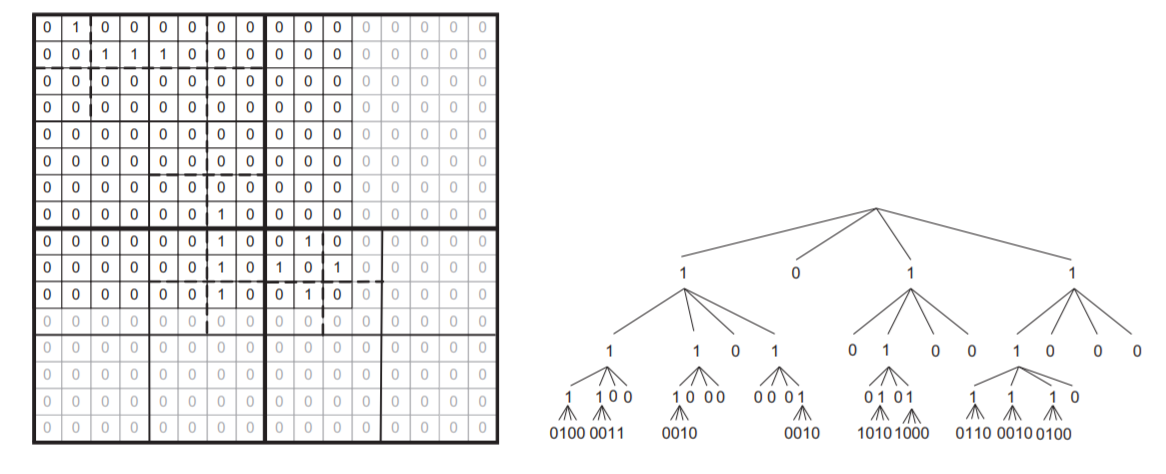
\includegraphics[height=200 pt, width=450 pt]{./ressources/image/k2-trees.png} 
\end{center}
\caption{Exemple de représentation $k^2$-trees d'une matrice d'adjacence d'un graphe}
\label{k2-trees-exemples}
\end{figure}


Pour le stockage de l'arbre, l'algorithme utilise deux tableaux de bits : un tableau T (Tree) contenant tous les nœuds de l'arbre à l'exception du dernier niveau et un tableau L (Leaves) contenant les feuilles du dernier niveau. Les nœuds et les feuilles sont ordonnés selon un parcours en largeur de l'arbre.   
Ci-dessous les deux tableaux T et L de l'exemple précédent (figure \ref{k2-trees-exemples}) : \\
T = 1011 1101 0100 1000 1100 1000 0001 0101 1110\\
L = 0100 0011 0010 0010 1010 1000 0110 0010 0100\\
Dans le pire des cas, l'espace totale pour la description de la structure est $k^2$m($log_{k^2}\frac{n^2}{m}$+ \textit{O}(1)), où n est le nombre de nœuds du graphe et m le nombre de liens. Cependant, pour les graphe du monde réel, l'espace nécessaire pour le stockage est bien meilleur. \\

Dans le même travail \citep{brisaboa2009k}, et dans le but d'obtenir un compromis entre la taille de l'arbre et le temps de parcours , les auteurs ont proposé une hybridation qui consiste a changer la valeur du paramètre k en fonction du niveau de l'arbre en donnant a k une grande valeur au début pour réduire le nombre de niveaux et améliorer ainsi le temps de recherche, et une petite valeur a la fin pour avoir des petites sous matrices et réduire l'espace de stockage.\\
Pour le stockage de l'arbre, un tableau $T_{i}$ est utilisé pour chaque valeur $k_{i}$, le tableau L reste le même.\\

Plusieurs variantes de l'algorithme de base ont été proposés dans la littérature dont le but était soit d'obtenir un meilleur résultat de compression, soit d'appliquer la méthode sur d'autres types de graphes. Nous allons dans ce qui suit présenter les travaux qu'on a put trouver.\\

Dans \citep{shi2012optimizing}, les auteurs proposent deux techniques d'optimisation de l'algorithme : la première consiste à trouver un certain ordre de nœuds qui permet de regrouper les 1 de la matrice d'adjacence dans une seule sous matrice au lieu qu'ils soient dispersés de manière aléatoire. La recherche d'un ordre optimal des nœuds est inenvisageable, avec k=2, le problème peut être réduit à un autre problème (min bisection) qui est NP-difficile, et quand k est dynamique le problème est plus compliqué. Comme solution, les auteurs utilisent DFS avec des heuristiques pour trouver une approximation de l'ordre optimal. Cette optimisation permet de réduire le nombre de nœuds internes et produire ainsi un arbre optimal. la deuxième optimisation est de trouver la valeur de k la plus adéquate pour chaque nœud interne, calculer cette valeur pour chaque nœud peut engendrer un temps de calcul très important. Pour éviter cela, les auteurs affectent la même valeur k pour les nœuds ayant le même parent. 	

Dans \citep{brisaboa2014compact}, les auteurs apportent deux amélioration principales dans le but d'optimiser l'espace et le temps de parcours de l'arbre produit : la première est de construire $k^2$ arbres distincts pour les $k_{0}^{2}$ sous matrices du premier niveau, cella à plusieurs avantages, premièrement, l'espace est réduit étant donné que la taille de chaque arbre est en fonction de $\frac{n^2}{k^2}$,deuxièmement le temps de parcours s'améliore puisque T et L sont plus petits. la deuxième amélioration est la compression de L qui consiste à construire un vocabulaire \textit{V} de tous les sous matrices du dernier niveau sous forme de séquences de bits, les classer par fréquence d'apparition et remplacer leurs occurrence dans L par des pointeurs, cela permet d'éviter la redondance et réduire par suit la taille de la structure. Les pointeur sont représenté par des codes de longueur variable ordonné, le plus petit correspond a la sous matrice la plus fréquente. Néanmoins, cette représentation ne permet  pas un accès direct dans L étant donné qu'une décompression séquentiel est nécessaire pour récupérer une position, pour remédier à ce problème les auteurs utilisent le principe de Directly Addressable Codes (DACs) \citep{brisaboa2013dacs} pour garantir un accès rapide au pointeur et conserver ainsi une navigation efficace.\\
Exemple : Pour la figure \ref{k2-trees-exemples}, le vocabulaire et L sont représentés comme suit :\\
\textit{V}= [0010 0100 0011 1010 1000 0110]\\
L = $c_{1}c_{2}c_{0}c_{0}c_{3}c_{4}c_{5}c_{0}c_{1}$ \\

\subsubsection{d$k^2$-trees}
Dans \citep{brisaboa2012compressed}, les auteurs développent la représentation $k^2$-trees pour les graphes dynamique. Ils proposent une nouvelle structure nommé d$k^2$-trees pour dynamique $k^2$-trees qui offre les même capacités de compression et fonctionnalités de navigation que le cas statique et qui permet également d'avoir des mises à jour sur le graphe. Pour atteindre ces objectifs, d$k^2$-trees remplace la structure statique de $k^2$-trees par une implémentation dynamique. Dans cette nouvelle implémentation, les deux tableaux T et L sont replacé par deux arbre, nommés $T_{tree}$ et $L_{tree}$ respectivement. Les feuilles de $T_{tree}$ et $L_{tree}$ stockent des parties des bitmaps T et L. La taille des feuilles est une valeurs paramétré. Les noeuds interns des deux arbres permettent d'accéder au feuilles et  de les modifier.\\
Chaque nœud interne de $T_tree$ contient 3 éléments : deux compteurs b et o qui contiennent respectivement le nombre de bits et le nombre de uns stocké dans les feuilles descendantes de ce nœud, un pointeur P vers le nœud fils. Les nœuds internes de $L_{trees}$ sont similaires sauf qu'ils ne contiennent que b et P. Avec cette structuration, $T_{tree}$ et $L_{tree}$ permettent l'ajout et la suppression des liens dans le graphe.\\
La figure \ref{dk2-trees} présente une représentation d$k^2$-trees : 

\begin{figure}[H]
\begin{center}
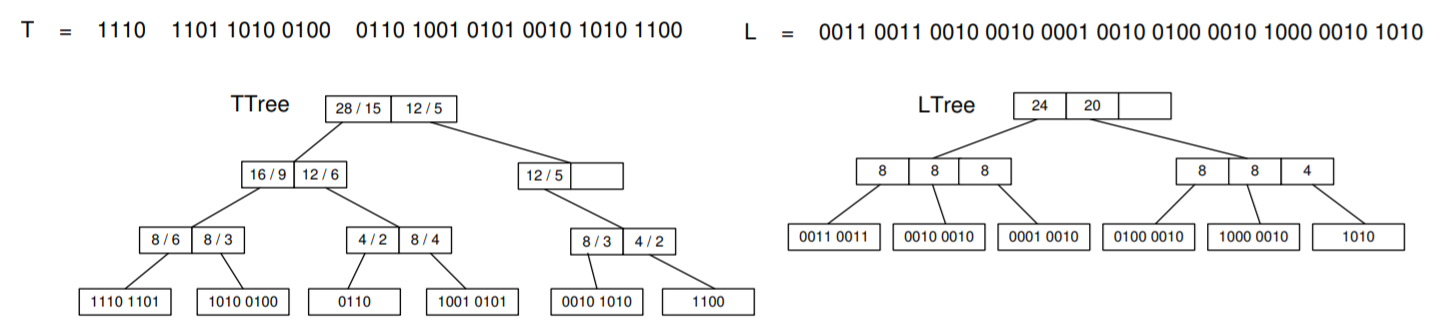
\includegraphics[height=100 pt, width=380 pt]{./ressources/image/dk2-trees.png} 
\end{center}
\caption{Exemple d'une représentation d$k^2$-trees}
\label{dk2-trees}
\end{figure}

\subsubsection{$k^n$-trees}
Dans \citep{de2013compact}, Sandra and al présente $k^n$-trees, une généralisation des $k^2$-trees pour les problème multidimensionnelles. Cette méthodes a plusieurs applications, elle est utilisé pour représenter les bases de donnés multidimensionnels, les rasters et les graphes dynamique. $k^n$-trees repose sur $k^2$-trees pour représenter une matrice à n-dimensions, la matrice est décomposer en $k^n$ sous-matrice de même taille, comme suit : Sur chaque dimension, K-1 hyperplans devise la matrice dans les position i$\frac{n}{K}$,pour $i \in [1, K-1]$. Une fois les dimensions partitionnés, $k^n$ sous-matrice sont induites, elles sont représenter  par des nœuds dans l'arbre comme dans l'algorithme de base. Les structure utilisés pour le stockage sont aussi les même (T et L).\\
En posant n=3, la méthode peut être appliqué sur les graphe dynamique ou temporelles. Ce type de graphes est représenter par une grille à 3 dimension $X \times Y \times T$, où les deux premières dimensions représentent les nœuds de départ et de destination, et la troisième dimension représente le temps. Une telle représentation peut facilement être stocker avec $k^3$-trees.
La figure \ref{kn-trees} présente une représentation $k^3$-trees d'un graphe dynamique :

\begin{figure}[H]
\begin{center}
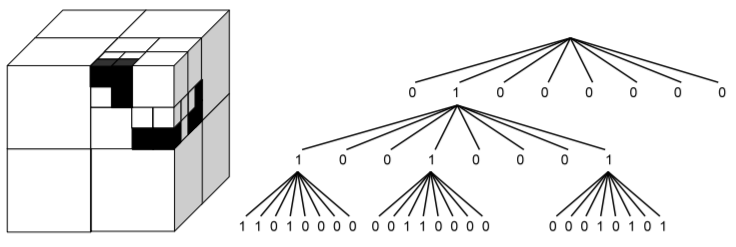
\includegraphics[height=100 pt, width=380 pt]{./ressources/image/kn-trees.png} 
\end{center}
\caption{Exemple d'une représentation $k^3$-trees}
\label{kn-trees}
\end{figure}



\subsubsection{$K^2$-tress1 }
Une autre variante de la méthode a été proposé par \citep{de2014new}. La représentation de base regroupe seulement les zones de zéros, puisque elle a été conçue au début pour les graphe du web qui possèdent une matrice d'adjacence extrêmement creuse. Les auteurs proposent d'étendre cette représentation en regroupant les zones de uns également. L'idée générale est d'arrêter la décomposition de la matrice d'adjacence quand une zone unis est trouvé, à savoir des zéros où des uns. Pour distinguer entre les différents nœuds, une représentation quadtree est utilisée \citep{de1997computational} : une couleur est attribué à chaque nœud, blanc pour une zone de zéro, noir pour une zone de uns et gris pour les nœuds internes e.i. les zones contenant des uns et des zéros. Pour le stockage des nœuds, les auteurs ont proposé quatre encodages présenter par la suite : \\

\textbf{ $k^2$-$trees1^{2-bits-naive}$ :} Dans cet encodage, deux bits sont utilisés pour représenter chaque type de nœud. L'attribution des bits n'est pas arbitraire, le premier bit du poids fort indique si le nœud est un nœud interne (0) ou une feuille (1), le deuxième détermine si les feuilles sont blanches (0) où noires (1). Nous aurons donc : 10 pour les nœuds gris, 01 pour les nœuds noir et 00 pour les nœuds blancs. Notant que les feuilles du dernier niveau sont représenter par un seule bit.
Après le codage, les premier bits de chaque nœud sauf ceux du dernier niveau sont stocker dans T, un autre tableau T' est créer pour sauvegarder les deuxièmes bits, les nœuds du dernier niveau sont stocker dans L.

\textbf{ $k^2$-$trees1^{2-bits}$ :} Le même principe de l'encodage précédant sauf que les nœuds gris sont représenter par un seul bit, toujours à 1, le tableau T' va contenir dans ce cas la couleur des feuilles, cela va réduire la taille de la structure.

\textbf{ $k^2$-$tree1s^{DF}$ :} Cet encodage est similaire à $k^2$-$trees^{2-bits}$, mais il utilise un seul bit pour les nœuds blancs et 2 bits pour les nœuds noirs et gris, compte tenue de la fréquence des nœuds blanc dans les graphe du monde réel par rapport au autres. Nous aurons donc : 0 pour les noeuds blancs, 10 pour les nœuds gris et 11 pour les nœuds noir.

\textbf{ $k^2$-$trees1^{5-bits}$ :} le dernier encodage repose sur la représentation de base, un nœud blanc est représenté par 0, un nœud noir où gris par 1, exactement comme le $k^2$-trees d'origine. Pour identifier un nœud noir (zone de uns), il sera représenté par une combinaison impossible : $k^2$ fils de 0 sont ajouté au nœud noir pour le distinguer.


La figure \ref{k2-trees1-exemple} illustre une représentation $k^2$-tress1 avec les quatre encodage : 


\begin{figure}[H]
\begin{center}
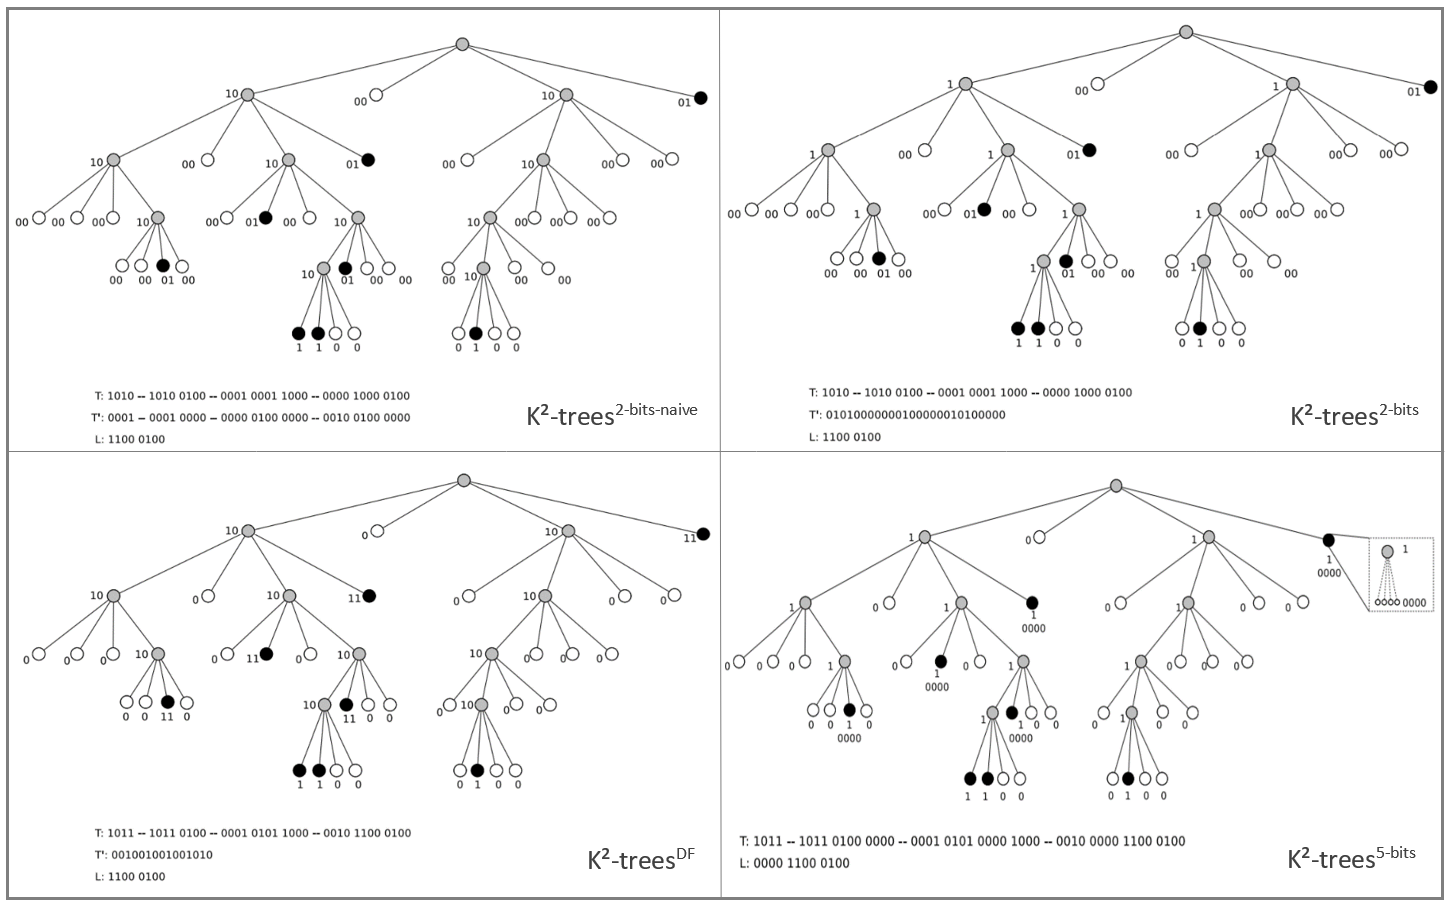
\includegraphics[height=300 pt, width=450 pt]{./ressources/image/k2-trees1.png} 
\end{center}
\caption{Exemple de représentation $k^2$-trees1 d'une matrice d'adjacence d'un graphe}
\label{k2-trees1-exemple}
\end{figure}


\subsubsection{Delta-$K^2$-tress }

Dans \citep{zhang2014delta}, les auteur proposent Delta-$k^2$-trees, une variante qui exploite la propriété de similarité entre les nœuds voisins du graphe pour réduire le nombre de uns dans la matrice d'adjacence. Notons par \textit{Matrix} la matrice d'adjacence, Delta-$k^2$-trees construit une nouvelle matrice appelé \textit{Delta-matrix}, une ligne \textit{i} de \textit{Delta-matrix} va contenir la différence entre les deux lignes \textit{Matrix}[i] et  \textit{Matrix}[i-1] si cela décroit le nombre de uns sinon elle sera égale à \textit{Matrix}[i]. e.i. : \\

$\left\{
\begin{array}{llcl}
Delta-matrix[i] & := matrix[i] & si & count1s(matrix[i]) < countDif(matrice[i],matrix[i-1]) \\
Delta-matrix[i] & := matrix[i] \bigoplus matrix[i-1] &  sinon
\end{array}
\right.$\\

Où count1s compte le nombre de 1 dans une ligne, countDif compte le nombre de bits différent entre deux ligne et $\bigoplus$ représente le ou exclusif.\\
Pour déterminer si une ligne est identique a celle de la matrice d'adjacence, un tableau D est utilisé : Si D[i]=1 la ligne est identique ,sinon elle est une ligne de différence.\\
La matrice \textit{Delta-matrix} contient moins de uns que la matrice d'adjacence, d'où elle est plus creuse, ce qui permet de réduire la taille de la structure et avoir un meilleur taux de compression. Cependant le temps de parcours est plus grand car pour accéder a certains lignes (lignes de différence), le graphe doit être décompresser et la matrice d'adjacence reconstituer\\

La figure \ref{k2-trees-delta} présente un exemple de la représentation Delta-$k^2$-trees


\begin{figure}[H]
\begin{center}
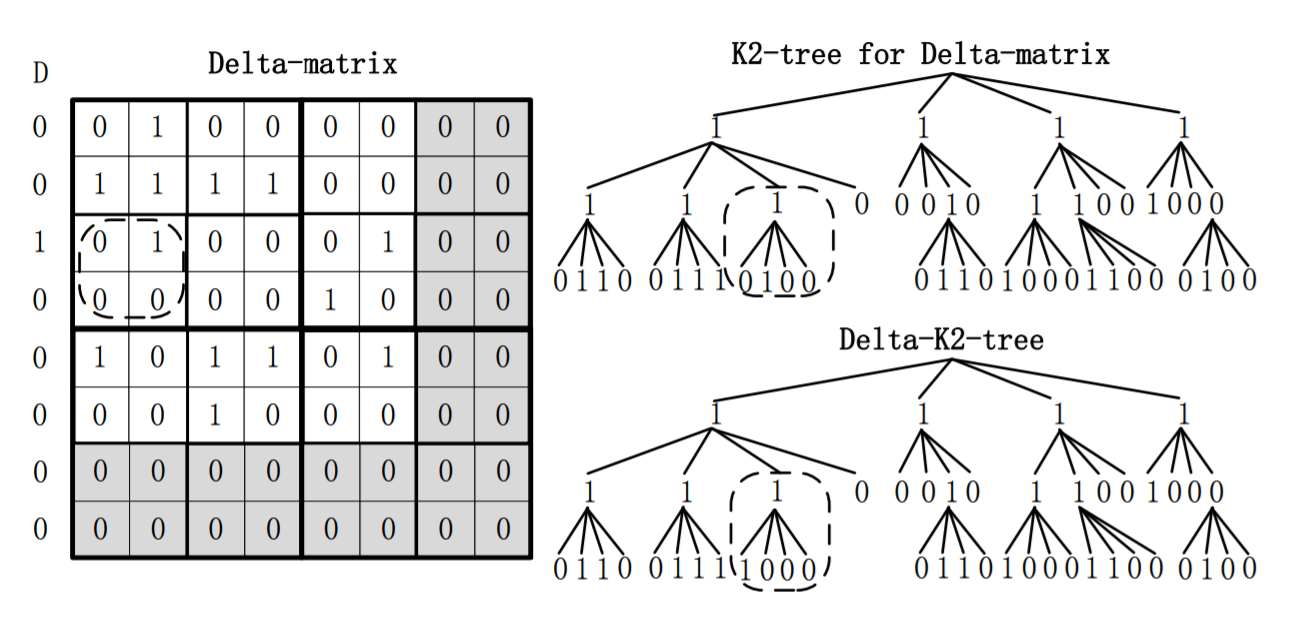
\includegraphics[height=150 pt, width=380 pt]{./ressources/image/k2-trees-delta.png} 
\end{center}
\caption{Exemple de représentation Delta-$k^2$-trees d'une matrice d'adjacence d'un graphe}
\label{k2-trees-delta}
\end{figure}

\subsubsection{$K^2$-treaps }
$K^2$-treaps est une autre variante de $k^2$-trees,elle a été proposé dans \citep{brisaboa2014k}. Cette variante combine les $k^2$-trees avec une autre structure de donnés appelé treaps \citep{aragon1989randomized}, les auteurs applique cette méthode sur des grilles multidimensionnels comme OLAP pour pouvoir les stocker et répondre efficacement aux requêtes top-K \citep{badr2013traitement}. La méthode peut être également appliqué sur les graphe pondéré, où chaque case de la matrice d'adjacence du graphe comporte le poids de l'arrêt qu'elle représente au lieu d'un 1.
Une décomposition récursive en $k^2$ sous-matrice est appliqué sur la matrice d'adjacence et un arbre $k^2$-air est construit comme dans l'algorithme de base, comme suit : la racine de l'arbre va contenir les coordonnés de la cellule avec le plus grands poids de la matrice, ainsi que sa valeur. La cellule qui vient d'être ajouté à l'arbre est ensuite supprimé de la matrice. Si plusieurs cellules ont la même valeurs maximales, l'une d'elles est choisis au hasard. Ce processus est répété récursivement sur chaque sous matrice en choisissant la cellule la plus lourde qu'elle contient pour la représenter dans l'arbre avec ses coordonnés et sa valeurs, et supprimer la cellule choisis au final. La procédure contenue sur chaque branche de l'arbre jusqu'à ce qu'on tombe sur les cellules de la matrice d'origine où sur une sous matrice complètement vide.\\
La figure \ref{k2-treaps} suivante illustre le représentation $k^2$-treaps d'un graphe pondéré \citep{badr2013traitement} :

\begin{figure}[H]
\begin{center}
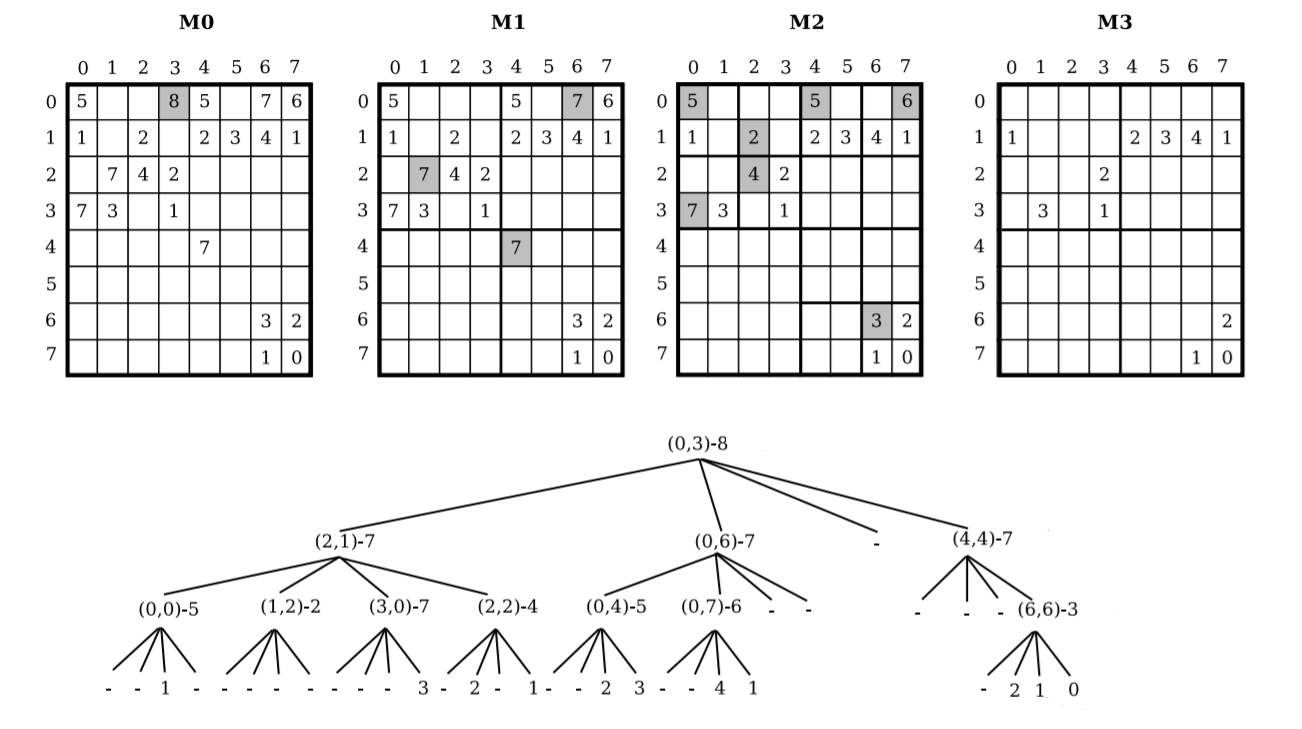
\includegraphics[height=200 pt, width=380 pt]{./ressources/image/k2-treaps.png} 
\end{center}
\caption{Exemple de représentation $k^2$-treaps d'une matrice d'adjacence d'un graphe pondéré}
\label{k2-treaps}
\end{figure}

\textbf{Structure de donnés :} Pour avoir une bonne compression, $k^2$-treaps effectue des transformation sur les donnés stockés . La première transformation consiste a changer les coordonné  représenté dans l'arbre en des coordonné relative par rapport a la sous matrice actuelle, la deuxième est de remplacer chaque poids dans l'arbre par la différence entre sa valeur et celle de son parent.\\
Trois structures de donnés sont utilisés pour sauvegarder les coordonnés et les valeurs des cellules ainsi que la topologie de l'arbre. Chaque structure est détaillé dans ce qui suit :
\begin{itemize}
\item \textit{Listes de coordonnés locales :} la séquence de coordonnés de chaque niveau \textit{l} de l'arbre est stocké dans une liste \textit{coord}[\textit{l}].
\item \textit{liste des valeurs : } Le parcours de l'arbre se fait en largeur, la séquence de valeurs récupéré est stocké dans une liste nommé \textit{values}. Un tableau nommé \textit{first} est utilisé pour sauvegarder la position de commencement de chaque niveau dans \textit{values}.
\item \textit{L'arbre :} la structure de l'arbre $k^2$-treaps est sauvegarder avec un arbre $k^2$-trees, les nœuds contenant des valeur dans $k^2$-treaps sont représenter par des uns, les nœuds vides par des zéros. Pour le stockage de l'arbre, un seul tableau T est utilisé. 
\end{itemize}

La figure \ref{k2-treaps-structure} représente les structures de donnés utilisés pour le stockage de l'arbre de la figure \ref{k2-treaps} précédente \citep{badr2013traitement} :

\begin{figure}[H]
\begin{center}
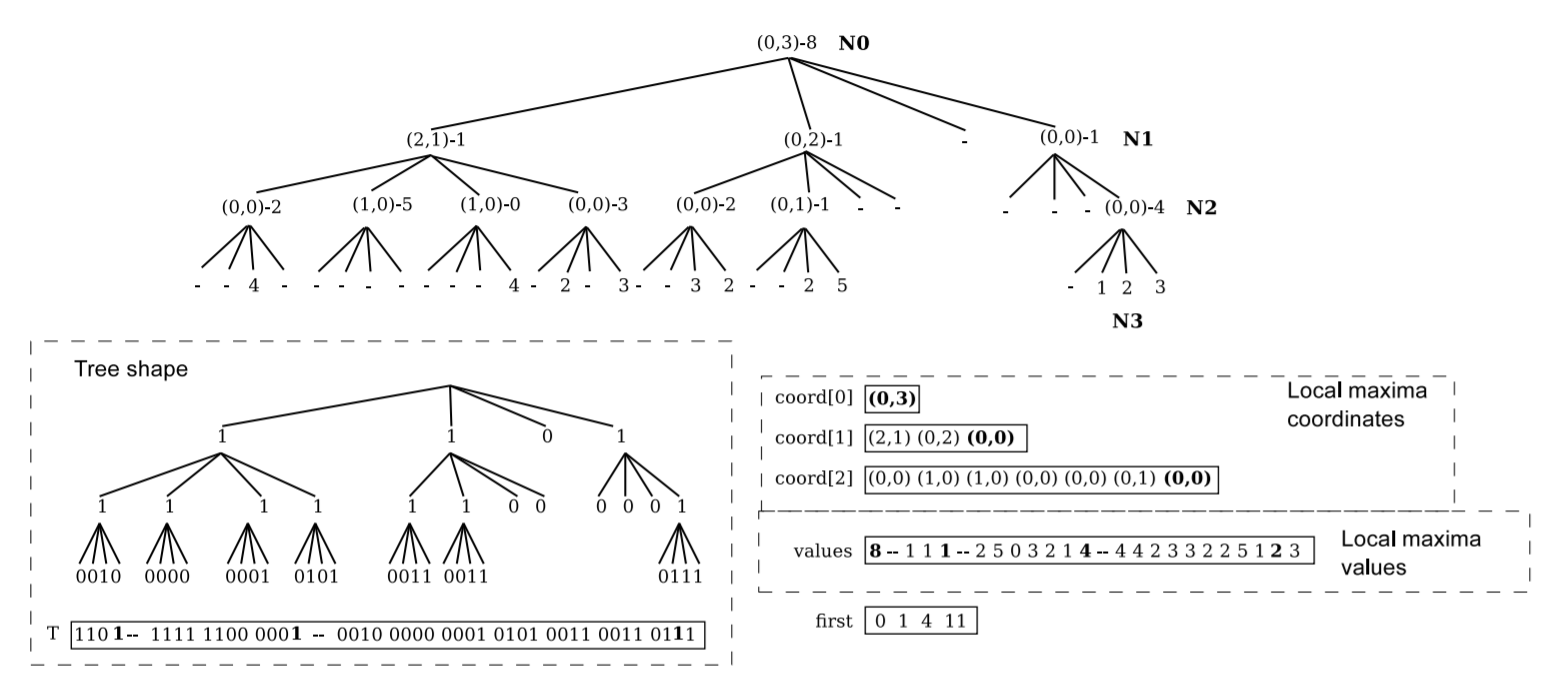
\includegraphics[height=200 pt, width=380 pt]{./ressources/image/k2-treaps-structure.png} 
\end{center}
\caption{Structures de donnés pour une représentation $k^2$-treaps d'une matrice}
\label{k2-treaps-structure}
\end{figure}

\subsubsection{I$k^2$-trees}
Une autre représentation a été proposé par \citep{garcia2014interleaved}, intitulé I$k^2$-trees pour Interleaved $k^2$-trees, Elle est appliqué sur les bases de donnés RDF ainsi que sur les graphe dynamique. Les auteurs proposent cette méthodes pour les relations ternaires, Une relation ternaire est définit par un triplet T=\{ $x_i$,$y_j$,$t_k$ \} $\subseteq$ $ X \times Y \times T$, I$k^2$-trees transforme cette relation en |Z| relation binaire . Dans les graphe dynamique, les deux premières dimension correspondent aux nœuds sources et destination et la troisième dimension reflète le temps. Le graphe est donc définit par |T| matrices d'adjacence prise à des instants $t_k$ différents. I$k^2$-trees représente les matrices simultanément, chaque matrice est représenté par un arbre $k^2$-trees, les arbre sont par la suit regroupé dans un seul arbre. Chaque nœuds de l'arbre obtenue représente une sous-matrice comme dans l'algorithme de base, sauf qu'au lieu d'utiliser un seule bit, I$k^2$-trees utilise 1 à |T| bits pour représenter le nœud. Le nœud racine contient |T| bits. Le nombre de bits de chaque fils est donné par le nombre de uns de son parent. l'arbre final est stocké comme dans l'original $k^2$-trees avec deux tableau : T et L.\\
La figure \ref{Ik2-trees} est un exemple de I$k^2$-trees appliqué sur un graphe dynamique représenté sur trois instants

\begin{figure}[H]
\begin{center}
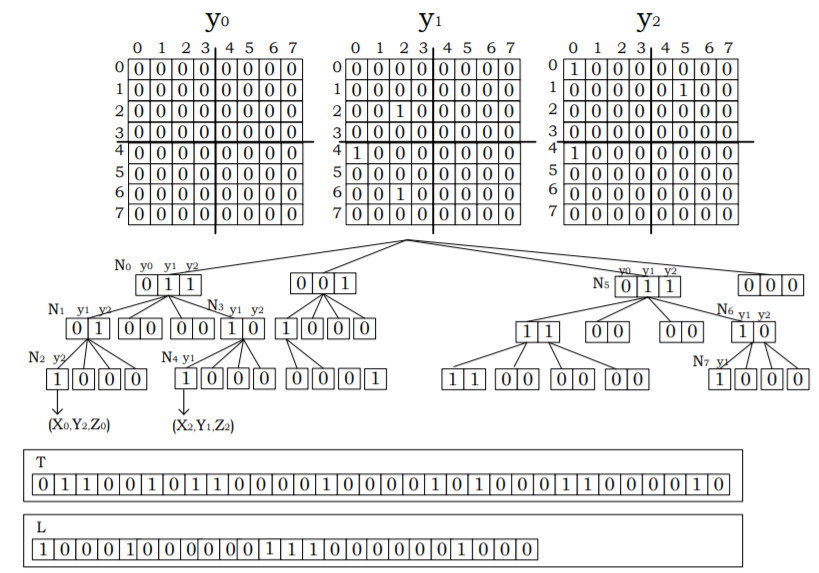
\includegraphics[height=200 pt, width=380 pt]{./ressources/image/Ik2-trees.png} 
\end{center}
\caption{Exemple d'une représentation I$k^2$-trees}
\label{Ik2-trees}
\end{figure}

\subsubsection{diff I$k^2$-trees}
Une variante de I$k^2$-trees appelé Differential I$k^2$
-tree a été étudié dans \citep{alvarez2017succinct}, son but est d'améliorer le taux de compression en représentant uniquement les changements survenue sur le graphe à un instant $t_i$ au lieu d'une instance complète : A l'instant $t_0$, une capture complète du graphe (matrice d'adjacence) est stocké. A l 'instant $t_k$, pour k>0, seuls les arrêtes qui change de valeurs entre $t_{k-1}$ et $t_k$ sont stockés. Les matrices sont représenter a la fin de la même manière que I$k^2$-trees. La limite de cette représentation est que la structure doit être décompresser lors d'une requêtes. \\
La figure \ref{Ik2-trees-diff} montre un exemple d'une représentation diff I$k^2$-trees.

\begin{figure}[H]
\begin{center}
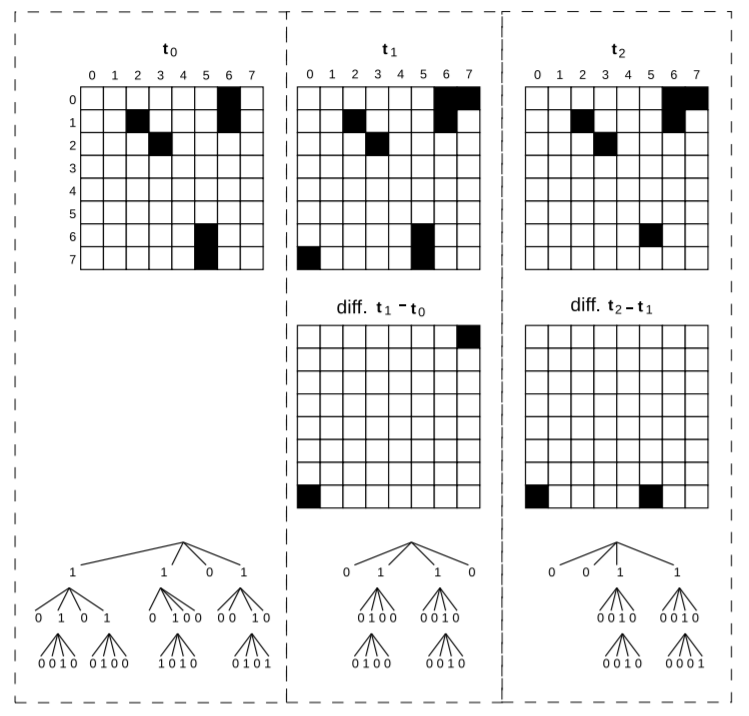
\includegraphics[height=200 pt, width=380 pt]{./ressources/image/Ik2-trees-diff.png} 
\end{center}
\caption{Exemple d'une représentation diff I$k^2$-trees}
\label{Ik2-trees-diff}
\end{figure}

\subsubsection{Att $K^2$-trees }
Dans \citep{alvarez2018compact}, les auteurs étendent la représentation $k^2$-trees pour les bases de donnés orienté graphe. Ces graphes sont étiquetés, attribués, orientés et ont des arrêtes multiples. Ils présentent le graphe sous forme d'une nouvelle structure intitulé Att $k^2$-trees pour Attributed $k^2$-trees.\\
La figure \ref{k2-trees-att-graphe} montre un exemple de graphe pris en compte par Att $K^2$-trees

\begin{figure}[H]
\begin{center}
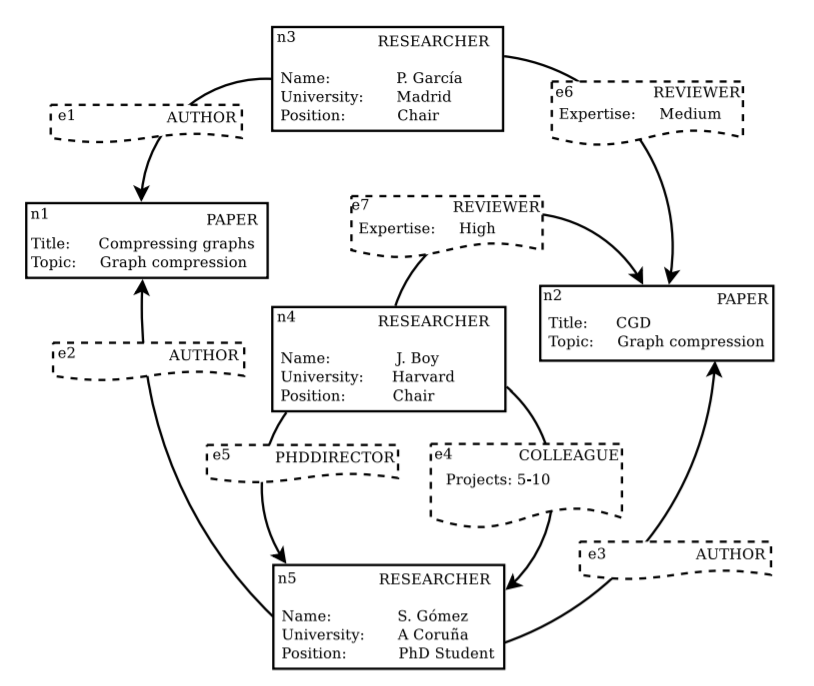
\includegraphics[height=200 pt, width=280 pt]{./ressources/image/k2-trees-att-graphe.png} 
\end{center}
\caption{Exemple d'un graphe étiqueté, attribué, orienté et multiple}
\label{k2-trees-att-graphe}
\end{figure}

\textbf{Structures de donnés :} La représentation obtenue par la compression est composer d'un ensemble d'arbres $k^2$-trees et d'autres structures supplémentaires. Le graphe est représenter par trois composants : un schéma de donnés, les donnés incluse dans les nœuds et les liens et finalement la relation entre les éléments du graphe. Chaque composant est présentés dans ce qui suit :
\begin{itemize}
\item \textit{Schéma : } Ce composant gère les étiquette et les attribues de chaque type d'éléments, il joue le rôle d'un indexe dans la représentation. Il est composé de :
\begin{description}
\item[Un schéma de nœuds :] représenter par un tableau qui contient les étiquètes des nœuds du graphe ordonné lexicographiquement. Un identifiant est attribué a chaque nœud du graphe selon l'ordre du tableau, les \textit{$m_1$} possédant la première étiqueté du tableau vont avoir des identifiant de 1 à \textit{$m_1$}, les \textit{$m_2$} nœuds avec la deuxième étiquette du tableau vont avoir des identifiants de \textit{$m_1$}+1 à \textit{$m_1$}+\textit{$m_2$} et ainsi de suit. chaque entrée du tableau va stocké  le plus grand identifiant portant son étiquette, cela permet de trouver l'étiquette d'un nœud a travers son identifiant.
\item[Un schéma d'arrêtés :] Comme dans le cas des nœuds, un tableau est utilisé pour stocker les étiquette des arrêtes avec le même principe.  
\end{description}
Le schéma est le point de départ de la représentation, il permet d'obtenir l'étiquette d'un nœud ou d'une arrêt, et d'accéder a ses attributs.
\item \textit{Donnés :} Ce composant contient tous les valeurs que peut prendre un attribut dans le graphe. Un attribut peut être représenter de deux façons différentes selon sa fréquence d'apparition, on distingue donc deux type d'attributs :
\begin{description}
\item[Attributs rares :] Ce sont les attributs qui prennent généralement des valeurs différentes a chaque apparition, ils sont stocker dans des listes et indexer avec l'identifiant de l'élément.
\item[Attributs fréquents :] Ce type d'attributs est sauvegarder dans deux matrices, une pour les attributs des nœuds et l'autre pour les attributs des liens. les matrices sont stocker sous forme d'arbres $k^2$-trees.
\end{description}
La figure \ref{k2-trees-att-schema} illustre les deux composants schéma et donnés de la représentation Att$k^2$-trees  de la figure \ref{k2-trees-att-graphe} précédente
\begin{figure}[H]
\begin{center}
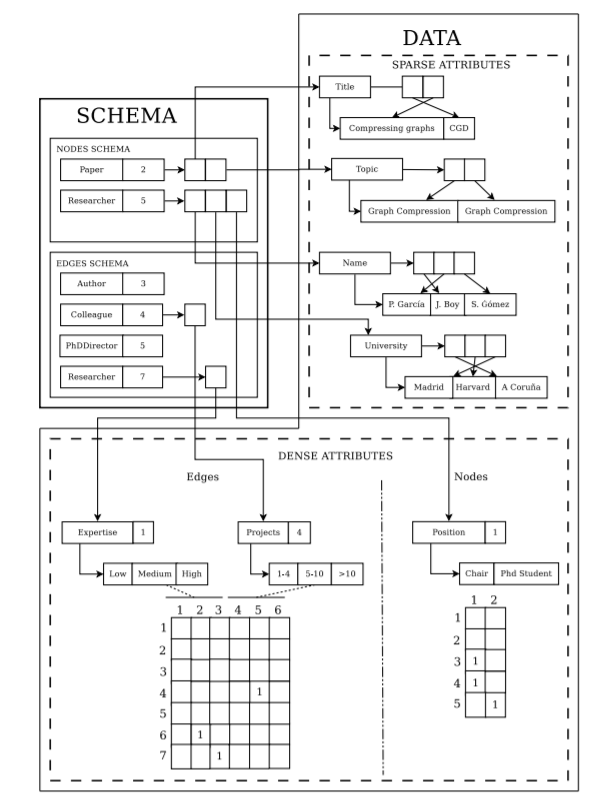
\includegraphics[height=200 pt, width=280 pt]{./ressources/image/k2-trees-att-schema.png} 
\end{center}
\caption{Exemple d'un schéma et donnés de la représentation Att$k^2$-trees}
\label{k2-trees-att-schema}
\end{figure}


\item \textit{Relations :} C'est le dernier composant de Att$k^2$-trees, il stocke les relations entre les nœuds et les arrêtes du graphe en utilisant un arbre $k^2$-trees et d'autres structures pour sauvegarder les identifiants des arrêts ainsi que les arrêtes multiples. Les structures supplémentaires sont les suivants :
\begin{description}
\item[Multi :] Un tableau qui indique si l'arrête est multiple où non.
\item[Firt :] Un Tableau qui donne l'identifiant de l'arrêt, où de celui de la première dans le cas d'une arrête multiple.
\item[Next :] Un tableau qui contient les identifient des arrêtes multiples restantes.
\end{description}
La figure \ref{k2-trees-att-relation} donne la représentation Att$k^2$-trees des relations du graphe de la figure \ref{k2-trees-att-graphe} :
\begin{figure}[H]
\begin{center}
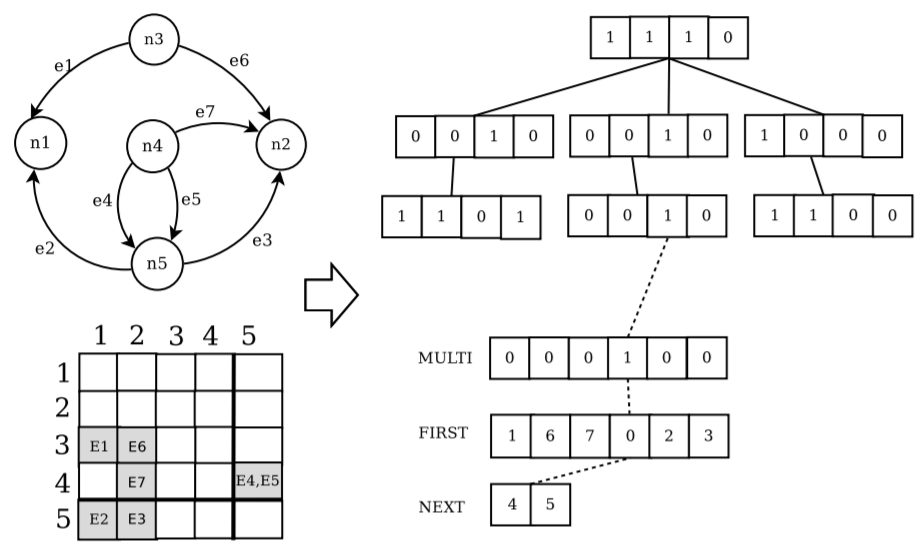
\includegraphics[height=200 pt, width=280 pt]{./ressources/image/k2-trees-att-relation.png} 
\end{center}
\caption{représentation des relations dans Att$k^2$-trees}
\label{k2-trees-att-relation}
\end{figure} 
\end{itemize}

\subsubsection{dynAtt$k^2$-trees }
Dans le même article \citep{alvarez2018compact}, les auteurs étendent Att$k^2$-trees pour les graphes dynamiques, il proposent une nouvelle variante appelé dynAtt$k^2$-trees qui supporte le changement dans les attributs et les liens du graphe. Comme Att$k^2$-trees, dynAtt$k^2$-trees représente le graphe avec trois composants : Schémas, donnés et relations. Les composants sont semblables a ceux de Att$k^2$-trees mais avec certaines amélioration vue la nature dynamique du graphe.\\
\textbf{Structure de donnés : } 
\begin{itemize}
\item \textit{Schéma :}  En ce qui concerne les nœuds, leurs étiquettes sont stockés dans une liste dynamique ordonné lexicographiquement. En outre, une séquence dynamique est utilisé pour sauvegarder le type de chaque nœud, elle est stocké ensuite sous forme d'un arbre d'ondelettes \citep{grossi2003high}. Le même principe est appliqué sur les arrêtes. 
\item \textit{Données :} Les attributs rares sont stockés dans des listes dynamiques, quant aux attributs fréquents, ils sont sauvegardé avec des arbres d$k^2$-trees (un arbre pour chaque attribut).
\item \textit{Relations :} Le stockage des relations se fait à l'aide d'un d$k^2$-trees et des tableaux dynamiques pour stockés les identifiants des arrêtes et les arrêtes multiples.
\end{itemize}




























		
		\section{Conclusion}


%---->chapitre 03 :« Etude empirique »
	\chapter{chapitre 03: etude empirique}

	\begin{defn}
			Here is a new definition
		\end{defn}
	

%Conclusion Générale									Obligatoire
\part{Conclusion} 

%Références Bibliographiques (fin de la pagination)		Obligatoire

%Annexes													Selon besoin
Random citation \citep{seo2018effective} embeddeed in text.

Random citation \citep{brisaboa2009k} embeddeed in text.

\newpage
\bibliography{Bibliographie}
\bibliographystyle{apalike}
\end{document}

%\renewcommand{\thefigure}{\arabic{figure}}
%\setcounter{figure}{0}
%\begin{figure}[H]
%	\centering
%	\includegraphics[scale=1]{ressources/image/LAAS-2016.jpg}
%	\label{fig:figure1}
%	\caption{This is a teste of figure}
%\end{figure}